% SMPC 2019 proceedings
% remember to compile twice in LaTeX, then with make Index, then with LaTeX again, twice.

\documentclass[10pt, twoside]{book}
\usepackage[utf8]{inputenc}
\usepackage[T1]{fontenc}
\usepackage{multicol}
\usepackage{setspace}
\usepackage{graphicx}
\usepackage{wrapfig}
\usepackage{mathptmx}  % Use times font for text and math
\usepackage{fancyhdr}
\usepackage{makeidx}
\usepackage{pdfpages}
\usepackage{hyperref}
\usepackage{geometry}
\usepackage{tipa}
\usepackage[labelformat=empty]{caption}
\usepackage{array}
\usepackage{enumitem}
\usepackage{float}
\usepackage[section]{placeins}
\usepackage{helvet}

% formatting commands
% defining table dimensions for talks (AB) and posters (DE) 
\newcolumntype{A}{>{\raggedleft\arraybackslash}m{2.5cm}}
\newcolumntype{B}{>{\arraybackslash}b{13.5cm}}
\newcolumntype{D}{>{\raggedleft\arraybackslash}m{1cm}}
\newcolumntype{E}{>{\raggedright\arraybackslash}b{13.5cm}}
% font
\renewcommand*\familydefault{\sfdefault}
% float placement
%\renewcommand*\textfraction{0.1}
\renewcommand*\floatpagefraction{0.99}
\geometry{inner=2.5cm,outer=2.5cm,top=2.3cm,bottom=2.3cm}
\pagestyle{fancy}
% colour schema for hyperlinks
\hypersetup{colorlinks=true, linkcolor=blue, filecolor=magenta, urlcolor=blue}
% fancy header details
\lhead[\thepage]{2019 Biennial Meeting of the Society of Music Perception and Cognition}
\rhead[New York University, August 5-7th, 2019]{\thepage}
\lfoot{}
\cfoot{}
% indexing FTW
\makeindex
\usepackage[totoc]{idxlayout}
\includepdfset{offset=0mm 0}
% pdfs
\pdfinclusioncopyfonts 1

% The Document itself
\begin{document}
%cover

\includepdf[pages=1,pagecommand=\thispagestyle{empty}]{cover_02b_program_small}%
%\includepdf{cover_02b_program_large}%

\tableofcontents

\newpage

\section*{Welcome Address}\addcontentsline{toc}{section}{Welcome Address}

It is our great pleasure to welcome you to the 2019 meeting of the Society for Music Perception and Cognition, hosted by New York University.  It's an exciting time for NYU, which has recently seen the development of new interdisciplinary endeavors in music and science.  The Music and Audio Research Laboratory (MARL), which originated as the research arm of the Music Technology Program at NYU and has music cognition as one of its focus areas, is now an official Center at NYU. This past spring, NYU and the Max Planck Institute for Empirical Aesthetics in Frankfurt established the Max Planck-NYU Center for Language, Music and Emotion (CLaME).  We're thrilled to be able to host SMPC 2019 at NYU and hope that both SMPC and the university will benefit from the potential research cross-pollination and collaboration opportunities that will arise from the conference events.
 
We had a record number of submissions this year, resulting in 156 talks, 164 posters, and 7 symposia on the program.  We are also excited to have a large international contingent, hailing from around the world.  Back by popular demand are the faculty-student lunches, as well as two early career panels.  There will also be a panel featuring journal editors and a seminar on applying to grad school.  We have two big social events planned: our opening reception on August 5 and a Circle Line dinner cruise around Manhattan on August 6.  As you experience the conference, please feel free to add your comments and reflections on the SMPC conference Facebook page and on Instagram and Twitter (\#smpc2019).
 
You will also notice a shorter format for both the conference itself and the paper presentations compared to recent years. In order to make it financially accessible for as many attendees as possible, we limited the conference events to three days and secured dorm housing to help reduce travel costs. We shortened the talk time slots to 15 minutes to allow us to remain inclusive in the more limited time frame. We also opted for a dinner cruise instead of a traditional banquet to provide an opportunity for SMPC attendees to experience New York City while connecting with each other in a more open social format. 
 
This conference would not be possible without the help of the many colleagues and administrative staff who contributed to all aspects of the conference.  We are able to present a diverse and extensive program thanks to our 88-person scientific committee and meta-reviewers, whose contributions made it possible to assign three reviews per submission.  Special thanks also to the administrative and technical staff in the Department of Music and Performing Arts Professions, the Steinhardt School, and the Kimmel Center, whose time and dedication have been crucial to the success of this conference.
\\
\\
Sincerely,
\\
\indent Mary Farbood and Johanna Devaney, Conference Chairs

Peter Martens, Program Chair

Finn Upham, Publicity and Publication Chair

\begin{figure}[H]
\centering
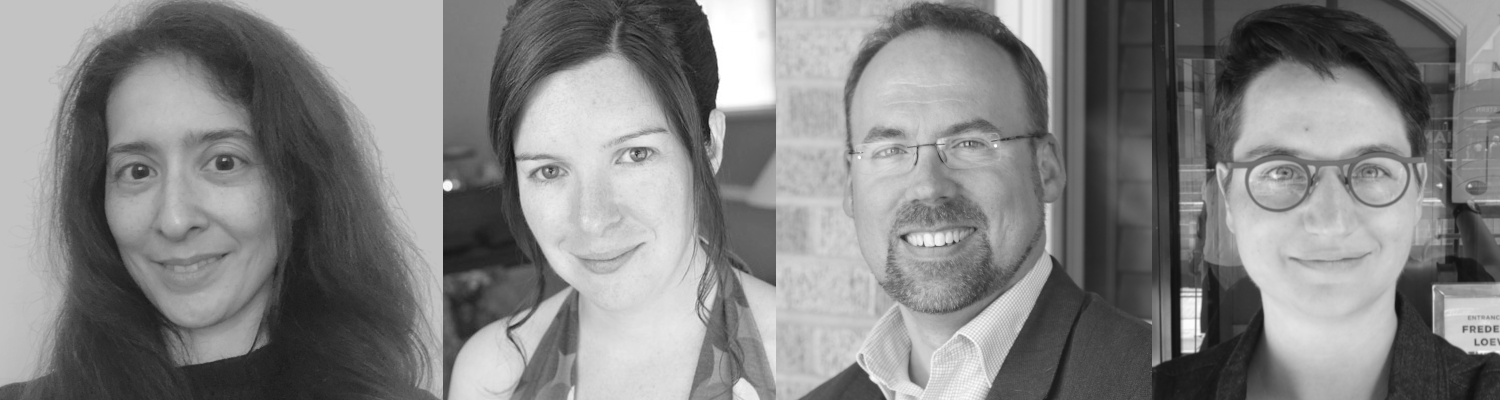
\includegraphics[width=1\linewidth]{images/Chairs_photo_2.png}
\end{figure}


\newpage
\singlespacing
% change itemize style? not dots
% make subsection titles centered?

\section*{Committees}\addcontentsline{toc}{section}{Committees}

\begin{multicols}{2}
\subsection*{Conference Organizers}
Morwaread Farbood, Conference Chair\\
\vspace{.5em}New York University\\
Johanna Devaney, Conference Chair\\
\vspace{.5em}Brooklyn College and CUNY Graduate Center\\
Peter Martens, Program Chair\\
\vspace{.5em}Texas Tech University\\
Finn Upham, Publication and Publicity Chair\\
\vspace{.5em}New York University

\subsection*{Conference Staff (NYU)}
Dirk Vander Wilt, Webmaster \\
Ryan Bloes, Lead Student Organizer\\
Ana DeJesus, Kimmel Center Events Coordinator

\subsection*{Department of Music and Performing Arts Professions Staff (NYU)}
Joshua Bailey, Registration \& Summer Programs\\
Thomas Beyer, Technology Supervisor\\
Tom Doczi, Recording Supervisor\\
Amy Fair, Administrative Director\\
Drew Francis, Event supervisor\\
Jenny Kuh, Administrative Aide\\
Debbie Nyarko, Special Projects Administrator\\
Christal Somar, Budget Administrator\\
Randy Susevich, Performance Venues \& Facilities\\
Michael Vince, Operations Administrator

\subsection*{Scientific Reviewers}
Mayumi Adachi\\
\vspace{.5em}Hokkaido University\\
Joshua Albrecht\\
\vspace{.5em}Kent State University\\
Vinoo Alluri\\
\vspace{.5em}IIIT - Hyderabad\\
Richard Ashley\\
\vspace{.5em}Northwestern University\\
Freya Bailes\\
\vspace{.5em}University of Leeds\\
Ramesh Balasubramaniam\\
\vspace{.5em}UC Merced\\
Amy Belfi\\
\vspace{.5em}Missouri University of Science and Technology\\
\\Jonathan Berger\\
\vspace{.5em}Stanford University\\
Tonya Bergeson\\
\vspace{.5em}Butler University\\
Marilyn G. Boltz\\
\vspace{.5em}Haverford College\\
Birgitta Burger\\
\vspace{.5em}University of Jyvaskyla\\
Blake Butler\\
\vspace{.5em}Western University\\
Daniel Cameron\\
\vspace{.5em}Western University\\
Peter A. Cariani\\
\vspace{.5em}Boston University\\
Charlie Chubb\\
\vspace{.5em}UCI\\
Laura K. Cirelli\\
\vspace{.5em}University of Toronto Scarborough\\
Daniel C. Comstock\\
\vspace{.5em}UC-Merced\\
Kathleen A Corrigall\\
\vspace{.5em}MacEwan University\\
Eugenia Costa-Giomi\\
\vspace{.5em}Ohio State\\
Lola Cuddy\\
\vspace{.5em}Queen's University\\
Meagan Curtis\\
\vspace{.5em}Purchase College, SUNY\\
Roger T. Dean\\
\vspace{.5em}Western Sydney University\\
Steven M. Demorest\\
\vspace{.5em}Northwestern University\\
W. Jay Dowling\\
\vspace{.5em}The University of Texas at Dallas\\
Tuomas Eerola\\
\vspace{.5em}Durham University\\
Hauke Egermann\\
\vspace{.5em}University of York\\
Zohar Eitan\\
\vspace{.5em}Tel Aviv University\\
Lauren Fink\\
\vspace{.5em}UC Davis\\
Clement Francois\\
\vspace{.5em}University of Barcelona\\
Ronald S. Friedman\\
\vspace{.5em}University at Albany, State University of New York\\
Takako Fujioka\\
\vspace{.5em}Stanford University\\
Bruno Gingras\\
\vspace{.5em}University of Innsbruck\\
Assal Habibi\\
\vspace{.5em}USC\\
Andrea Halpern\\
\vspace{.5em}Bucknell University\\
Erin Hannon\\
\vspace{.5em}UNLV\\
Frank Heuser\\
\vspace{.5em}UCLA\\
Michael Hove\\
\vspace{.5em}Fitchburg State University\\
Beatriz Ilari\\
\vspace{.5em}USC\\
John Iversen\\
\vspace{.5em}UCSD\\
Nori Jacoby\\
\vspace{.5em}Max Planck for Empirical Aesthetics\\
Blair Kaneshiro\\
\vspace{.5em}Stanford University\\
Alex Khalil\\
\vspace{.5em}UCSD\\
Sonja Kotz\\
\vspace{.5em}Maastrict University\\
Alexandra Lamont\\
\vspace{.5em}Keele University\\
Psyche Loui\\
\vspace{.5em}Northeastern\\
Elizabeth H Margulis\\
\vspace{.5em}Princeton University\\
Panayotis Mavromatis\\
\vspace{.5em}New York University\\
Devin McAuley\\
\vspace{.5em}Michigan State University\\
Lucy McGarry\\
\vspace{.5em}Western University\\
Carson G. Miller Rigoli\\
\vspace{.5em}UC San Diego\\
Daniel Mullensiefen\\
\vspace{.5em}Goldsmiths\\
Angela Nazarian\\
\vspace{.5em}UC Davis\\
Martin Norgaard\\
\vspace{.5em}Georgia State University\\
Mitch Ohriner\\
\vspace{.5em}Shenandoah University\\
Isabelle Peretz\\
\vspace{.5em}University of Montreal\\
Peter Pfordresher\\
\vspace{.5em}University at Buffalo\\
Jon Prince\\
\vspace{.5em}Murdoch University\\
Mark Reybrouck\\
\vspace{.5em}Leuven\\
Jessica M. Ross\\
\vspace{.5em}University of California, Merced\\
Frank Russo\\
\vspace{.5em}Ryerson University\\
Daniela Sammler\\
\vspace{.5em}Max Planck Institute, Human Cog. and Brain Sci.\\
Adena Schachner\\
\vspace{.5em}UCSD\\
Rebecca Schaefer\\
\vspace{.5em}Universiteit Leiden\\
Andrea Schiavio\\
\vspace{.5em}University of Graz\\
Mike Schutz\\
\vspace{.5em}McMaster\\
David Sears\\
\vspace{.5em}Texas Tech University\\
Kimberly Sena Moore\\
\vspace{.5em}University of Miami\\
Daniel Shanahan\\
\vspace{.5em}Louisiana State University\\
Robert Slevc\\
\vspace{.5em}University of Maryland\\
Joel Snyder\\
\vspace{.5em}UNLV\\
Laura Stambaugh\\
\vspace{.5em}Georgia Southern\\
Yi-Huang Su\\
\vspace{.5em}TU Munich\\
Siu-Lan Tan\\
\vspace{.5em}Kalamazoo College\\
Liila Taruffi\\
\vspace{.5em}Freie Universit{\"a}t Berlin\\
David Temperley\\
\vspace{.5em}Eastman School of Music\\
Mari Tervaniemi\\
\vspace{.5em}University of Helsinki\\
Renee Timmers\\
\vspace{.5em}University of Sheffield\\
Petri Toiviainen\\
\vspace{.5em}University of Jyv{\"a}skyl{\"a}\\
Laurel Trainor\\
\vspace{.5em}McMaster University\\
Sandra E. Trehub\\
\vspace{.5em}University of Toronto Mississauga\\
Christina Vanden Bosch der Nederlanden\\
\vspace{.5em}Western University\\
Leigh VanHandel\\
\vspace{.5em}Michigan State University\\
Dominique T. Vuvan\\
\vspace{.5em}Skidmore College\\
Matthew H. Woolhouse, McMaster University\\
Ted Zanto\\
\vspace{.5em}UCSF\\
Lawrence M. Zbikowski\\
\vspace{.5em}University of Chicago\\
Jennifer Zuk\\
\vspace{.5em}Harvard University

\subsection*{SMPC Board}
Elizabeth Hellmuth Margulis, President\\
Erin Hannon, Treasurer\\
Michael Schutz, Secretary\\
Amy Belfi, At-Large Board Member\\
Sarah Creel, At-Large Board Member\\
Petr Janata, At-Large Board Member\\
Robert Slevc, At-Large Board Member\\
Dominique Vuvan, At-Large Board Member\\
Psyche Loui, Media and Communications Chair\\
David Baker, Student Member

\subsection*{Supporting Organizations}
NYU Department of Music and Performing Arts \\
\indent Professions\\
NYU Steinhardt School of Culture, Education, and \\
\indent Human Development\\
Society for Music Perception and Cognition

\subsection*{Travel Award Recepients}
\textit{Congratulations to all the SMPC Travel Award Recipients for their excellent submissions}\\\\
\indent Tanushree Agrawal\\
\indent Gladys Heng\\
\indent Talia Liu\\
\indent Jessica Nave-Blodgett\\
\indent Tzu-Han Cheng\\
\indent Yeoeun Lim\\
\indent Neerjah Skantharajah\\
\indent Alissandra Reed\\
\indent Lindsay Warrenburg\\
%\indent Courtney Wilson
\end{multicols}

%% change itemize style? not dots
%% make subsection titles centered?
%
%\section*{Committees}\addcontentsline{toc}{section}{Committees}
%
%\begin{multicols}{2}
%\subsection*{Conference Organizers}
%%\begin{itemize}[label={}]
%%\item Conference Chair, Morwaread Farbood, New York University
%%\item Conference Chair, Johanna Devaney, Brooklyn College and CUNY Graduate Center
%%\item Program Chair, Peter Martens, Texas Tech University
%%\item Publication and Publicity Chair, Finn Upham, New York University
%%\end{itemize}
%
%Conference Chair, Morwaread Farbood, New York University\\
%Conference Chair, Johanna Devaney, Brooklyn College and CUNY Graduate Center\\
%Program Chair, Peter Martens, Texas Tech University\\
%Publication and Publicity Chair, Finn Upham, New York University\\
%
%\subsection*{Conference Volunteers and Support Staff}
%\begin{itemize}[label={}]
%\item Dirk Vander Wilt, conference webmaster
%\item Ryan Bloes, lead student organizer
%\item Joshua Bailey, registration site and summer programs administrator
%
%\end{itemize}
%
%\subsection*{Scientific Reviewers}
%\begin{itemize}[label={}]
%\item Mayumi Adachi, Hokkaido University
%\item Joshua Albrecht, Kent State University
%\item Vinoo Alluri, IIIT - Hyderabad
%\item Richard Ashley, Northwestern University
%\item Freya Bailes, School of Music, University of Leeds
%\item Ramesh Balasubramaniam, UC Merced
%\item Amy Belfi, Missouri University of Science and Technology
%\item Jonathan Berger, Stanford University
%\item Tonya Bergeson, Butler University
%\item Marilyn G. Boltz, Haverford College
%\item Birgitta Burger, University of Jyvaskyla
%\item Blake Butler, Western University
%\item Daniel Cameron, Western University
%\item Peter A Cariani, Boston University
%\item Charlie Chubb, UCI
%\item Laura K Cirelli, University of Toronto Scarborough
%\item Daniel C Comstock, UC-Merced
%\item Kathleen A Corrigall, MacEwan University
%\item Eugenia Costa-Giomi, Ohio State
%\item Lola Cuddy, Queen's University
%\item Meagan Curtis, Purchase College, SUNY
%\item Roger T. Dean, The MARCS Institute for Brain, Behaviour and Development, Western Sydney University
%\item Steven M. Demorest, Northwestern University
%\item W. Jay Dowling, The University of Texas at Dallas
%\item Tuomas Eerola, Durham University
%\item Hauke Egermann, University of York
%\item Zohar Eitan, Tel Aviv University
%\item Lauren Fink, UC Davis
%\item Clement Francois, University of Barcelona
%\item Ronald S Friedman, University at Albany, State University of New York
%\item Takako Fujioka, Department of Music, Center for Computer Research in Music and Acoustics, Stanford University
%\item Bruno Gingras, University of Innsbruck
%\item Assal Habibi, USC
%\item Andrea Halpern, Bucknell University
%\item Erin Hannon, UNLV
%\item Frank Heuser, UCLA
%\item Michael Hove, Fitchburg State University
%\item Beatriz Ilari, USC
%\item John Iversen, UCSD
%\item Nori Jacoby, Max Planck for Empirical Aesthetics
%\item Blair Kaneshiro, Stanford University
%\item Alex Khalil, UCSD
%\item Sonja Kotz, Maastrict University
%\item Alexandra Lamont, Keele University
%\item Psyche Loui, Northeastern
%\item Elizabeth H Margulis, Princeton University
%\item Peter A Martens, Texas Tech University
%\item Panayotis Mavromatis, NYU
%\item Devin McAuley, Michigan State University
%\item Lucy McGarry, Western University
%\item Carson G Miller Rigoli, UC San Diego
%\item Daniel Mullensiefen, Goldsmiths
%\item Angela Nazarian, UC Davis
%\item Martin Norgaard, Georgia State University
%\item Mitch Ohriner, Shenandoah University
%\item Isabelle Peretz, University of Montreal
%\item Peter Pfordresher, University at Buffalo
%\item Jon Prince, Murdoch University
%\item Mark Reybrouck, Leuven
%\item Jessica M Ross, University of California, Merced
%\item Frank Russo, Ryerson University
%\item Daniela Sammler, Max Planck Institute for Human Cognitive and Brain Sciences
%\item Adena Schachner, UCSD
%\item Rebecca Schaefer, Universiteit Leiden
%\item Andrea Schiavio, University of Graz
%\item Mike Schutz, Mcmaster
%\item David Sears, Texas Tech University
%\item Kimberly Sena Moore, University of Miami
%\item Daniel Shanahan, Louisiana State University
%\item Robert Slevc, University of Maryland
%\item Joel Snyder, UNLV
%\item Laura Stambaugh, Georgia Southern
%\item Yi-Huang Su, TU Munich
%\item Siu-Lan Tan, Kalamazoo College
%\item Liila Taruffi, Freie Universitat Berlin
%\item David Temperley, Eastman School of Music
%\item Mari Tervaniemi, University of Helsinki
%\item Renee Timmers, University of Sheffield
%\item Petri Toiviainen, University of Jyv{\"a}skyl{\"a}
%\item Laurel Trainor, McMaster University
%\item Sandra E Trehub, University of Toronto Mississauga
%\item Christina Vanden Bosch der Nederlanden, Western University
%\item Leigh VanHandel, Michigan State University
%\item Dominique T. Vuvan, Skidmore College \& International Laboratory for Brain, Music, and Sound Research
%\item Matthew H Woolhouse, McMaster University
%\item Ted Zanto, UCSF
%\item Lawrence M Zbikowski, University of Chicago
%\item Jennifer Zuk, Harvard University
%\end{itemize}
%
%\subsection*{SMPC Board}
%\begin{itemize}[label={}]
%\item Elizabeth Hellmuth Margulis, President
%\item Erin Hannon, Treasurer
%\item Michael Schutz, Secretary
%\item Amy Belfi, At-Large Board Member
%\item Sarah Creel, At-Large Board Member
%\item Petr Janata, At-Large Board Member
%\item Bob Slevc, At-Large Board Member
%\item Dominique Vuvan, At-Large Board Member
%\item Psyche Loui, Media and Communications Chair
%\item David Baker, Student Member
%\end{itemize}
%
%\subsection*{Supporting Organisations}
%\begin{itemize}[label={}]
%\item Department of Music and Performing Arts Professions
%\item NYU Steinhardt School of Culture, Education, and Human Development
%\item Society for Music Perception and Cognition
%\end{itemize}
%
%
%\subsection*{Travel Award Recepients}
%\textit{Congratulations to all the SMPC Travel Award Recipients for their excellent submissions}
%\begin{itemize}[label={}]
%\item Tanushree Agrawal
%\item Gladys Heng
%\item Talia Liu
%\item Jessica Nave-Blodgett
%\item Tzu-Han Cheng
%\item Yeoeun Lim
%\item Neerjah Skantharajah
%\item Alissandra Reed
%\item Lindsay Warrenburg
%\item Courtney Wilson
%\end{itemize}
%\end{multicols}
\newpage
\input{ConferenceInfo.tex}
\newpage

\section*{Conference Events}\addcontentsline{toc}{section}{Conference Events}
In addition to talks and poster sessions, there are several conference events that attendees are encouraged to attend.

\subsection*{Opening Reception}\addcontentsline{toc}{subsection}{Reception}
Following the Keynote and President's Address in Loewe Theater in August 5th, all attendees are welcome to the opening reception. Hors d'oeuvres, drink tickets, and a live jazz trio will be in the Rosenthal Pavilion, 10th floor of the Kimmel Center, starting at 6:45 PM.

\subsection*{Lunch Time Forums}\addcontentsline{toc}{subsection}{Lunchtime panels}
Three forums on aspect of academic life are scheduled during the lunch breaks:\\

\noindent  {\bf Grad Student Forum}\\
A panel of grad students and postdocs share their experience in navigating grad school via Q\&A, coordinated by SMPC student board member, David Baker.\\

\noindent  {\bf Early Career Forum}\\
 A panel  early career researchers share their experience getting established via Q\&A, coordinated by SMPC student board member, David Baker.\\

\noindent  {\bf Meet the Editors Panel}\\ 
This session will give an overview of trends in academic publishing with a focus on the journal {\it Music Perception}.  There will be time for Q\&A and an opportunity to meet some of the editors. Coordinated by Kate Steven, Editor of {\it Music Perception}.

\subsection*{Dinner Cruise}\addcontentsline{toc}{subsection}{Dinner Cruise}

The conference dinner cruise is on Tuesday evening. Ticket holders are encouraged to go directly from the last poster session to the port for boarding.\\ 

\noindent {\bf By Taxi}\\
Use the following address as the destination if hailing a taxi or Uber:\\
\indent Circle Line Sightseeing Cruises\\
\indent Pier 83, W 42nd St, New York, NY 10036\\

\noindent  {\bf By Subway}
\begin{itemize}
\item Walk to the W. 4th Street subway station. The closest entrance to this station from the Kimmel Center is on the corner of W. 3rd Street and 6th Avenue (5 minute walk).
\item Take an uptown (Manhattan or Queens-bound) A, C, or E train to Times Square 42nd St.
\item Navigate to 42nd Street from the subway station.
\item Walk towards 12th Avenue while traveling down 42nd Street. Pier 83 will be just past 12th Avenue on the Hudson River.
\end{itemize}
{\it Be sure to check the MTA homepage at} \url{https://new.mta.info} {\it to see if there are any service changes. An MTA worker will be available at W. 4th Street station should you have any questions or are in need of directions to Times Square}\\

\noindent  {\bf By Bus from Midtown}\\
From 42nd Street, take the M42 bus going West, directly to the Circle Line Pier. From 49th Street, take the M50 bus directly to the Circle Line Pier.



\newpage
\section*{Keynote}\addcontentsline{toc}{section}{Keynote}


The keynote address for SMPC 2019, \textit{Fire and Ice: A Case Study for the Sounds of Poetry Viewed as Music}, will be given by Fred Lerdahl, Professor Emeritus at Columbia University, in Loewe Theater at 5:30 PM on August 5th.


\subsection*{Abstract}

The sounds of poetry, like those of music, combine perceptually into hierarchically organized structures, making it possible to treat poetic sounds as if they were music. Using Ray Jackendoff's and my cognitively oriented music theory along with contemporary work in generative phonology, I explore this idea by developing a rule system that assigns to poetic lines the following structures: word groupings, stress and metrical grids, syllable durations, intonation contours, and hierarchical patterns of syllabic repetition and contrast. I illustrate these structures through an analysis of a short poem by Robert Frost, {\it Fire and Ice}. Three audio readings of the poem are compared to the analysis. In addition to providing a systematic method of poetic analysis, this study reveals structural features that poetry and music do and do not share. The talk closes with a presentation of my piece {\it Fire and Ice}, which is based in part on the foregoing poetic analysis and audio readings.

\subsection*{Biography}
\begin{wrapfigure}{r}{0.3\textwidth}
\centering
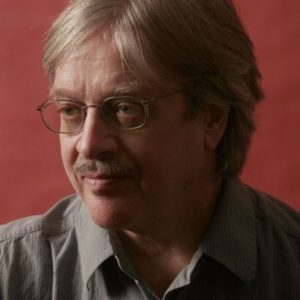
\includegraphics[width=1\linewidth] {images/lerdahl.jpg}
\end{wrapfigure}

Fred Lerdahl's music has been commissioned and performed by major chamber ensembles and orchestras in the United States and around the world, and he has been resident composer at leading institutions and festivals. His music is published by Schott Music Corporation and has been widely recorded for various labels including Bridge Records, which is producing an ongoing series of his music. Lerdahl is a member of the American Academy of Arts and Letters.

His seminal book {\it A Generative Theory of Tonal Music}, co-authored with linguist Ray Jackendoff, is a foundational document in the cognitive science of music. His second book, {\it Tonal Pitch Space}, which extends ideas from the earlier book, won the 2003 distinguished book award from the Society for Music Theory and an ASCAP-Deems Taylor award. A third book, {\it Composition and Cognition: Reflections on Contemporary Music and the Musical Mind}, based on his 2011 Bloch Lectures at UC/Berkeley, brings together his dual activity as composer and theorist; it will be published in November 2019. He has also published many articles in music theory and cognition, including ``Timbral Hierarchies,'' ``Cognitive Constraints on Compositional Systems,'' ``Atonal Prolongational Structure,'' and ``Modeling Tonal Tension'' (co-authored with music psychologist Carol Krumhansl).

Lerdahl studied at Lawrence, Princeton, and Tanglewood. He taught at UC/Berkeley, Harvard, and Michigan, and from 1991 to 2019 he was Fritz Reiner Professor of Musical Composition at Columbia, where he directed the composition program for 20 years.

\newpage
\section*{SMPC Code of Conduct}\addcontentsline{toc}{section}{SMPC Code of Conduct}


The Society for Music Perception and Cognition is dedicated to providing a harassment-free conference experience for everyone regardless of gender, gender identity and expression, sexual orientation, disability, physical appearance, body size, race, age or religion. We do not tolerate harassment of conference participants in any form. Sexual language and imagery is not appropriate for any conference venue, including talks. Conference participants violating these rules may be sanctioned or expelled from the conference at the discretion of the conference organizers. 

Harassment includes, but is not limited to:
\begin{itemize}
\item Verbal comments that reinforce social structures of domination (related to gender, gender identity and expression, sexual orientation, disability, physical appearance, body size, race, age, or religion)
\item Sexual images in public spaces
\item Deliberate intimidation, stalking, or following 
\item Harassing photography or recording
\item Sustained disruption of talks or other events
\item Inappropriate physical contact
\item Unwelcome sexual attention
\item Advocating for, or encouraging, any of the above behaviour
\end{itemize}

\subsubsection*{Enforcement}

Participants asked to stop any harassing behavior are expected to comply immediately. If a participant engages in harassing behaviour, event organizers retain the right to take any actions to keep the event a welcoming environment for all participants. This includes warning the offender or expulsion from the conference.

Event organizers may take action to redress anything designed to, or with the clear impact of, disrupting the event or making the environment hostile for any participants. We expect participants to follow these rules at all event venues and event-related social activities. We think people should follow these rules outside event activities too!

\subsubsection*{Reporting}

If someone makes you or anyone else feel unsafe or unwelcome, please report it as soon as possible. Harassment and other code of conduct violations reduce the value of the SMPC meeting for everyone. 

You can make a report either personally or anonymously.

\subsubsection*{Anonymous Report}

You can make an anonymous report by filling out the form at: \url{http://bit.ly/SMPC_report} 

We can't follow up an anonymous report with you directly, but we will fully investigate it and take whatever action is necessary to prevent a recurrence.

\subsubsection*{Personal Report}

You can make a personal report by emailing any of the SMPC Board members:
\begin{itemize}
\item Elizabeth Margulis (President): margulis@princeton.edu
\item Michael Schutz (Secretary): schutz@mcmaster.ca
\item Erin Hannon (Treasurer): erin.hannon@unlv.edu
\item Dominique Vuvan: d.vuvan@gmail.com
\item Amy Belfi: amybelfi@mst.edu 
\item Petr Janata: pjanata@ucdavis.edu 
\item Sarah Creel: screel@ucsd.edu
\item Bob Slevc: slevc@umd.edu 
\item Psyche Loui: p.loui@northeastern.edu 
\item David Baker (student representative): davidjohnbaker1@gmail.com 
\end{itemize}
When taking a personal report, we'll ask you to tell us about what happened. This can be upsetting, but you won't be asked to confront anyone and we won't tell anyone who you are.

SMPC leaders will be happy to help you contact hotel/venue security, local law enforcement, local support services, provide escorts, or otherwise assist you to feel safe for the duration of the event. We value your attendance.


\clearpage
% why is it so hard to get the table of contents to list this page correctly? still not quite.
\addcontentsline{toc}{section}{Condensed Schedule}
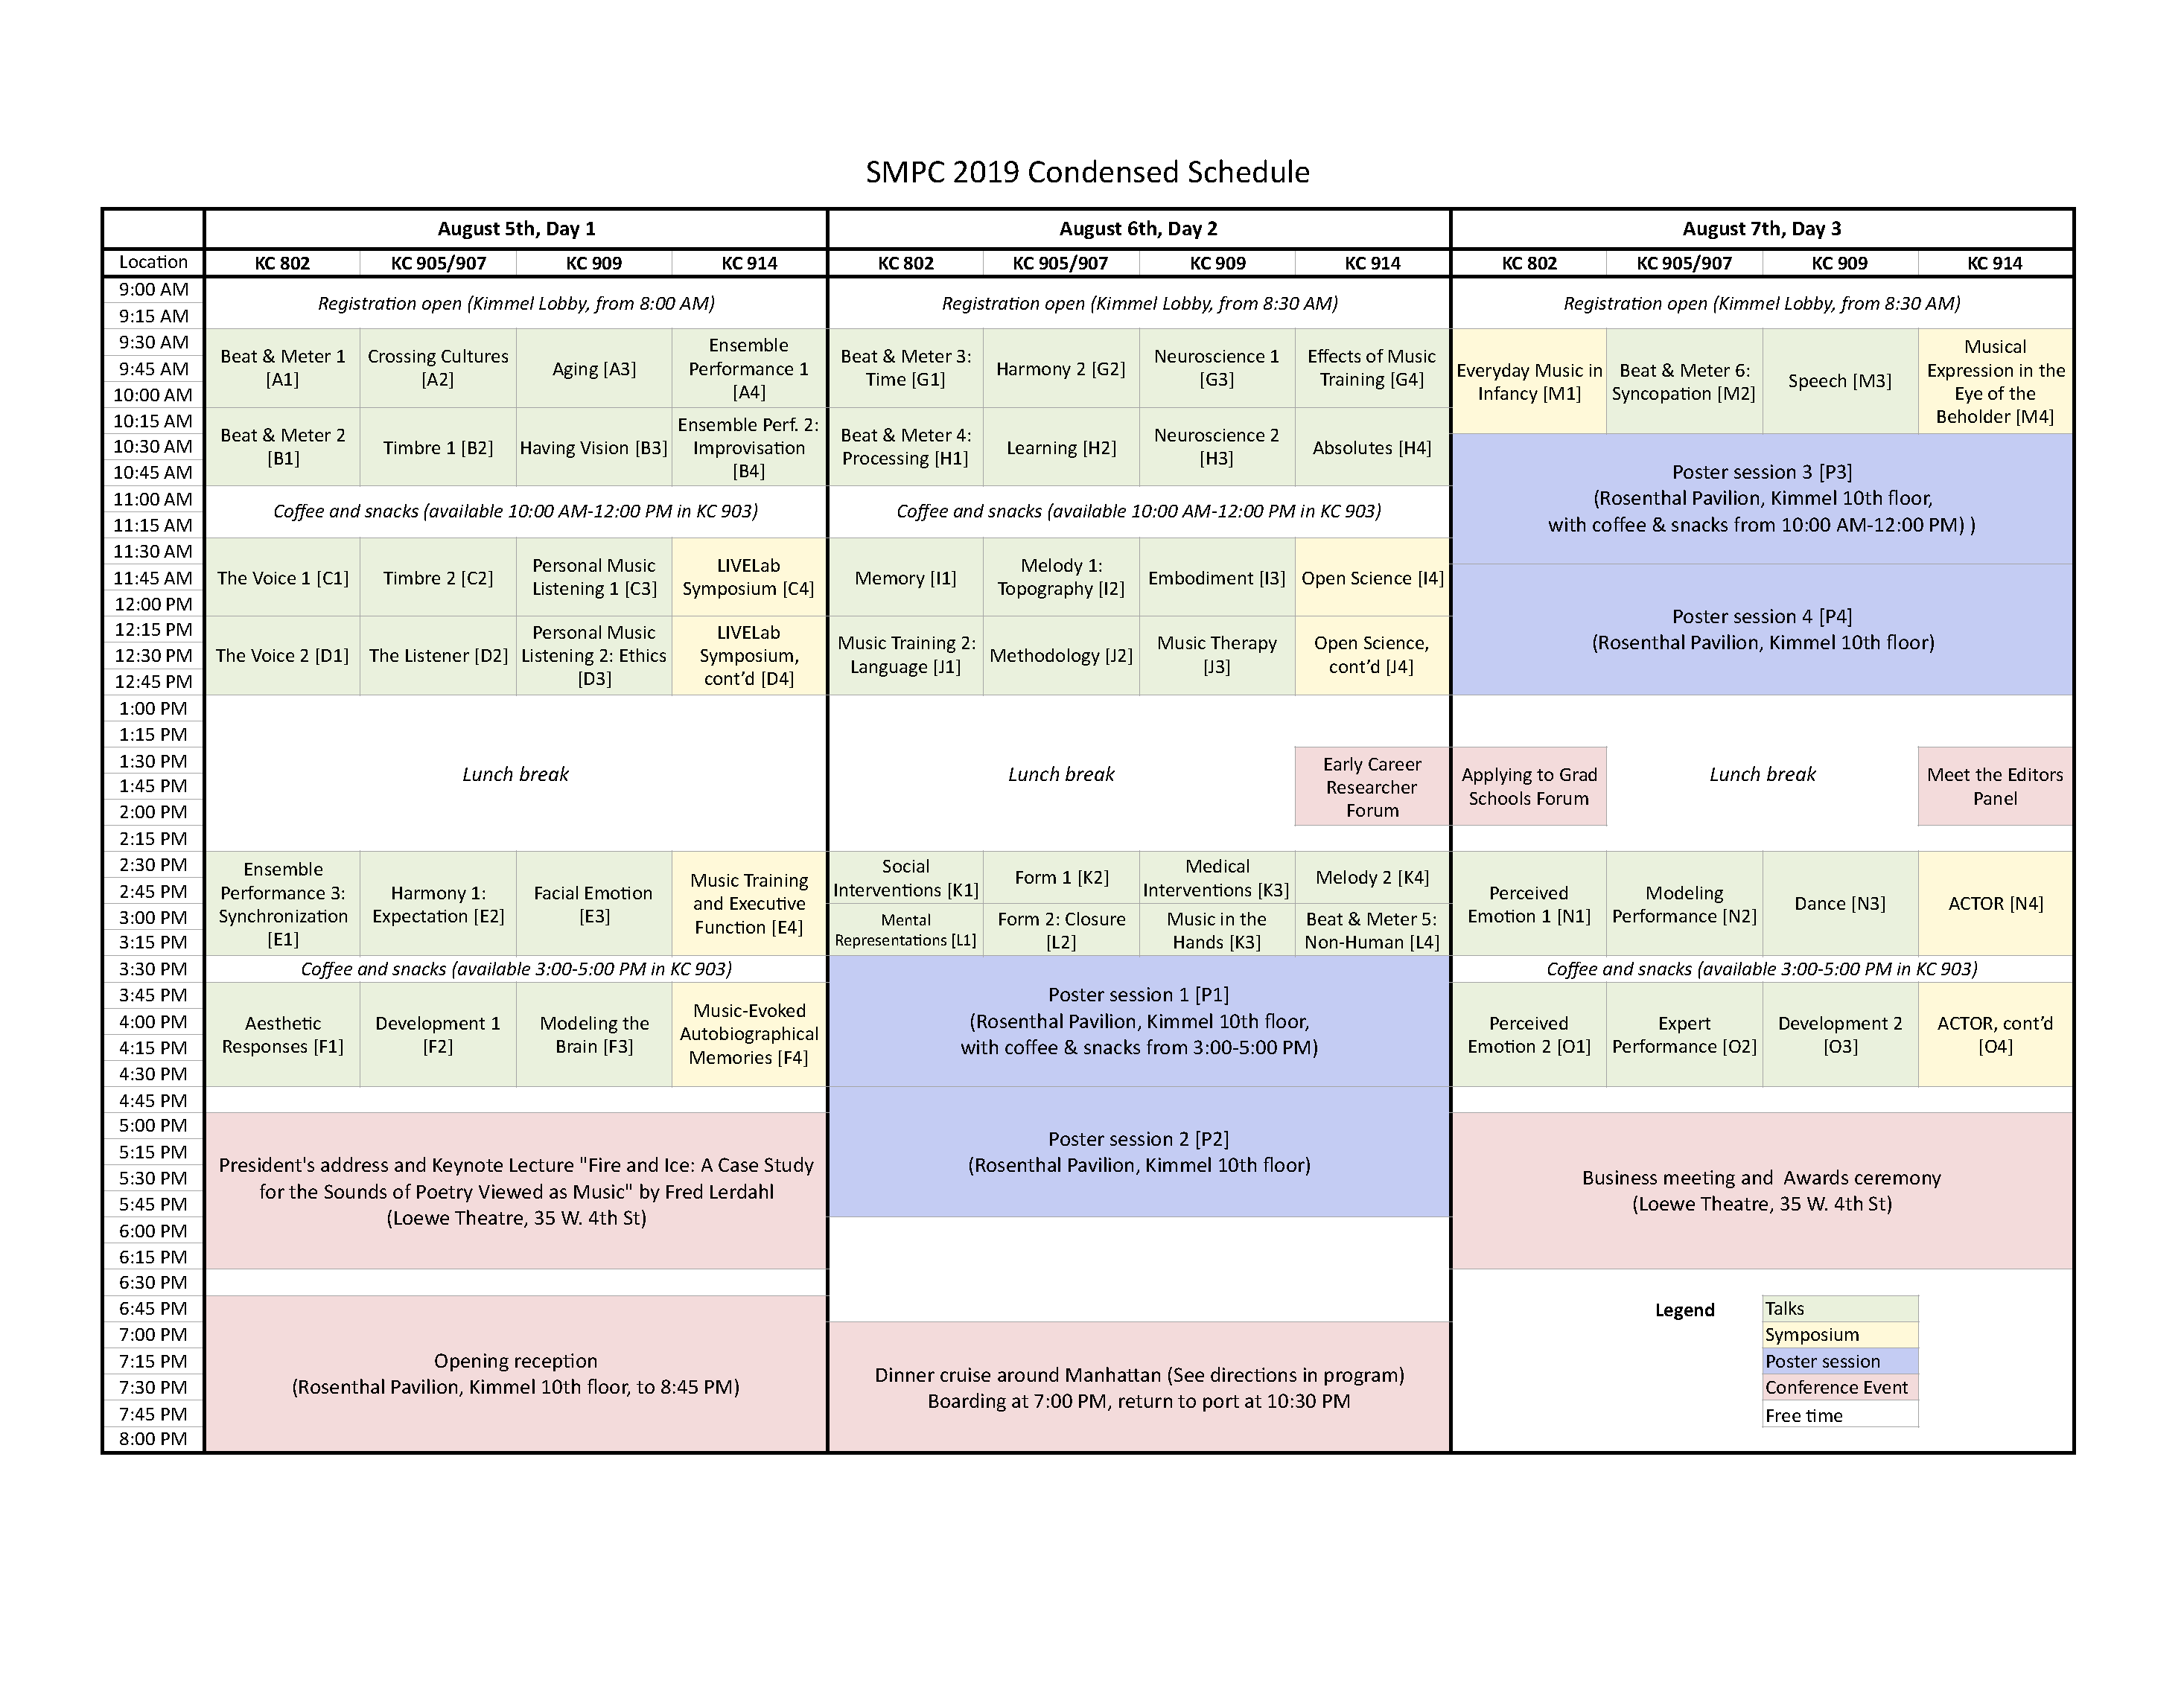
\includepdf[addtotoc={13,section,1,Condensed Schedule,schedule},angle=90,pages=1,pagecommand=\thispagestyle{empty}]{images/SMPC2019_Condensed_colour.pdf}%
\newpage

%Schedule details without abstracts, changing header along the way
\rhead[Presentations on Day 1, August 5, 2019]{\thepage}
\input{Aug5_Talks_Details.tex}
\newpage
\rhead[Presentations on Day 2, August 6, 2019]{\thepage}
\input{Aug6_Talks_Details.tex}
\input{Aug6_Poster_Details.tex}
\newpage
\rhead[Presentations on Day 3, August 7, 2019]{\thepage}
\input{Aug7_Talks_Details.tex}
\clearpage
\input{Aug7_Poster_Details.tex}

% last few pages of index and maps
\rhead[New York University, August 5-7th, 2019]{\thepage}
\clearpage
\printindex % note index is listed as component type Chapter, so it stands out in TOC, but that's OK.
\addcontentsline{toc}{section}{Maps}
\begin{wrapfigure}{r}{1\textwidth}
\centering
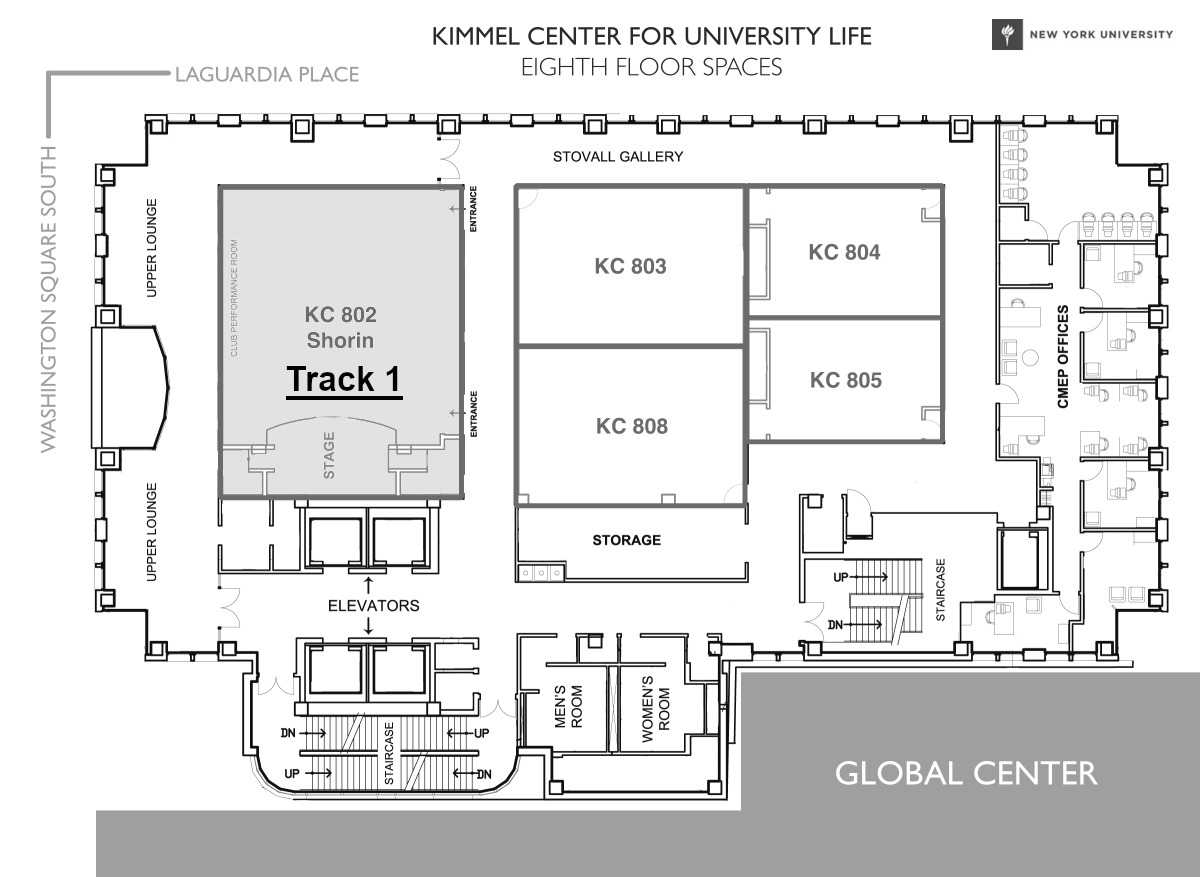
\includegraphics[width=1\linewidth] {images/KC_8th_floor_2.png}
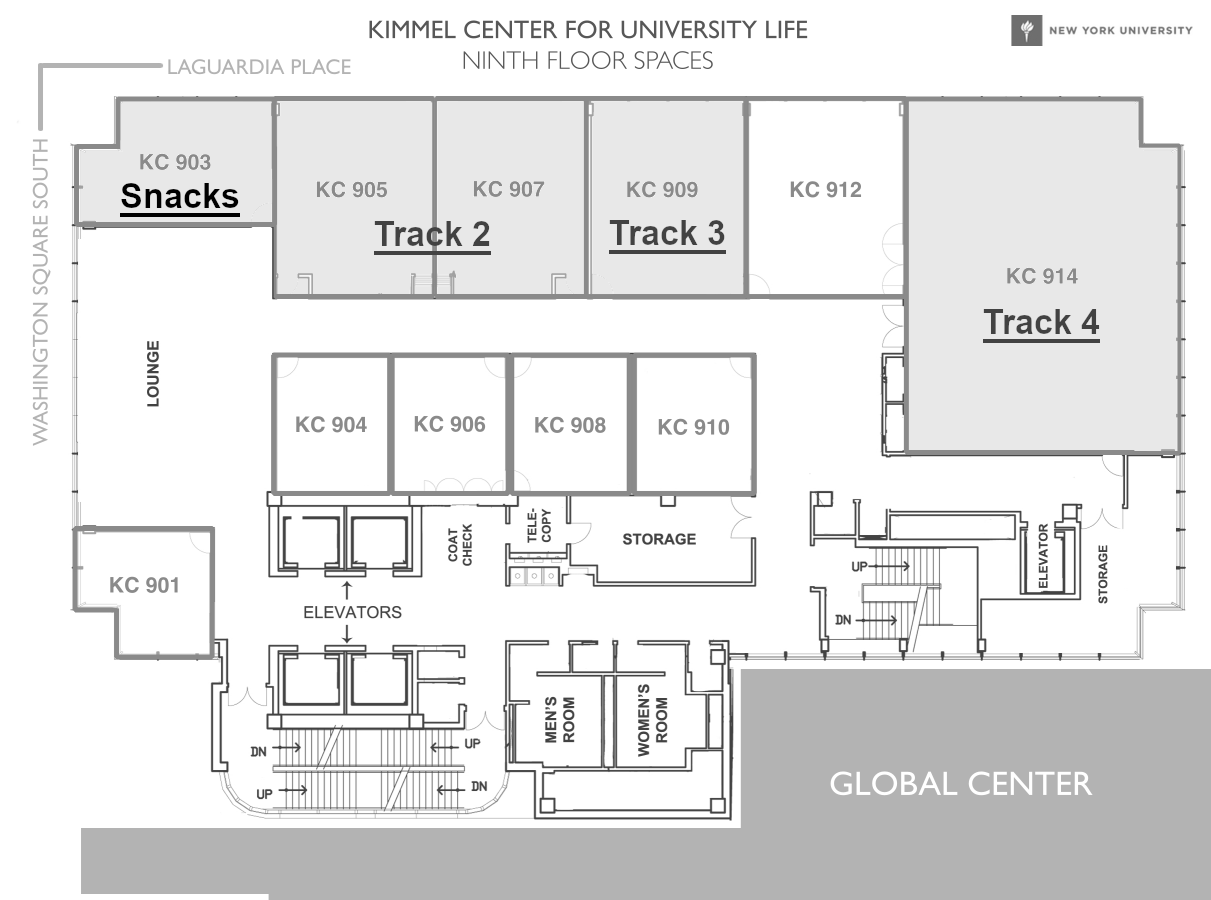
\includegraphics[width=1\linewidth] {images/KC_9th_floor_g.png}
\end{wrapfigure}

\begin{wrapfigure}{r}{1\textwidth}
\centering
\includegraphics[width=1\linewidth] {images/Large_area_map.eps}
\end{wrapfigure}

\end{document}